\section{Straighten the concepts}
\subsection{Discrepancy of usage of terms}

\begin{itemize}
    \item Most people don't share the same concepts and refer to things with the same name but refering to diferent things.
    \item People make up new names for new and old concepts.
    \item How long would it take for this phenomenon to cause disasters.
\end{itemize}

\section{Concepts as building blocks}
\Quote{Concepts, pretheoretically, are the constituents of thoughts}{Stanford Encyclopedia of Philosophy}


\subsection{Prerequisites for knowledge}
\begin{itemize}
    \item The two constituents of knoledge are: intuition and concepts.

    \Quote{Intuition and concepts constitute... the elements fo all our knowledge, so that neither concepts without an intuition in some way corresponding to them, nor intuition without concepts can yield knoledge}{Immanuel Kant 1724-1804}
    
    \item Concepts are illusive to grasp.

    \Quote{Nothing is more important than the formation of a fictional concept, which teach us at last to understand our own.}{Ludwig Wittgenstein 1889-1951}

    \item Most concepts are rooted deeply in us.

    \Quote{Our concept of governing is derived from our view of people. It is a concept deeply rooted in a set of beliefs firmlyy etched in the national conscience, of all of us.}{Barbara Jordan 1936-1996}
    Conceps are more or less constructs of human societies.

    \Quote{We coin concepts and we use them to analyse and explain nature and society. But we seem to forget, midway, that these concepts are our own constructs and start equating them with reality.}{Abdolkarim Soroush}
    
    \item Concepts $\neq $ reality, though concepts we understand reality.

    \Quote{Society exists only as a mental concept; in the real world there are only individuals.}{Oscal Wilde 1854-1900}

    
    \item Example:
        \begin{figure}[H]
            \centering
            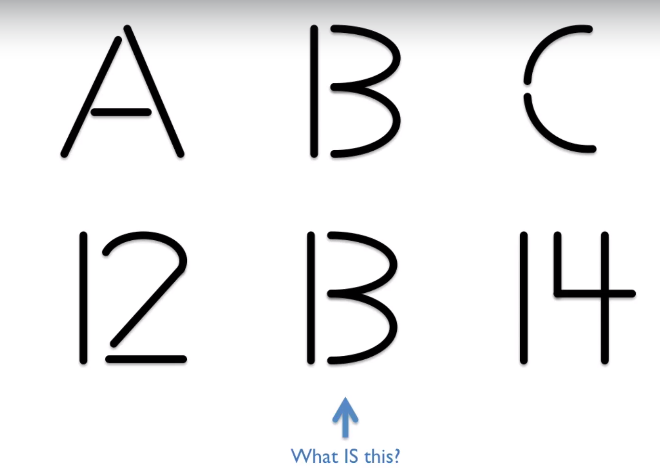
\includegraphics[]{Clases/figs/01.PNG} 
        \end{figure}
\end{itemize}


%%%%%%%%%%%%%%%%%%%%%%%%%%%%%%%%%%%%%%%%%%%%%%%%%%%%%%%%%%%%%%%%%%%%%%%%%%%%%%%%%%%%%%%%%%
\section{Visialization of concepts}
\begin{itemize}
    \item We can order concepts visually using maps.
    \item A conceptual map is a graphical tool that organizes and represents knoledge, it illustrates the concepts, also it shows the relationships between the concepts, it also labels the concept, specifies the relationship, this is to make a proposition.
    \item We use maps to boost concept learning, fast visualization of concepts, communicate better, to implement a better concept of our project.
    \item Creator of concept mapping: developed by Joseph Novak, initially used to analize view psycological phenomenon in kids.
    \item This is a tool that can be applicable to almost anything.
    \item It helps transform tactit information to explicit.
    \item Every big project starts out as a conceptual map.
    \item You can use conceptual maps to create etrics.
    \item Sumarry, concepts are:
        \begin{itemize}
            \item Concepts are the constituents of thoughts
            \item Visual tool 
            \item Boost knoledge acquisition, communication, system development and creativity.
            \item Applications are almost unlimited.
        \end{itemize}
    
    \item A conceptual map represents and organizes knoledge.
\end{itemize}


\section{Course goals and structure}
\begin{itemize}
    \item Introduction 
    \item Foundations 
    \item Notation - Models and UML 
    \item Process and workshop techniques 
    \item Packaging 
\end{itemize}


\section{Two ways to complete the course}
\begin{enumerate}
    \item Theory first: philosofical foundation and then notation.
    \item Practice first: learn the notation first and then the thory.
\end{enumerate}

